% =====================================================================
%  Research Statement -- Applied Mathematics (generic version)
%  Davood Damircheli, Department of Mathematics, Louisiana State University
%  Compile: pdflatex (twice)
%
%  Lines marked  %CHECK  contain claims that should be confirmed before
%  submission (authorship of in-preparation drafts, final numbers, etc.).
% =====================================================================
\documentclass[11pt]{article}
\usepackage[letterpaper,hmargin=1in,vmargin=0.85in]{geometry}
\usepackage[T1]{fontenc}
\usepackage{mathpazo}
\usepackage[scaled=0.95]{helvet}
\usepackage{microtype}
\usepackage{amsmath,amssymb}
\usepackage{xcolor}
\usepackage{enumitem}
\usepackage{titlesec}
\usepackage{tikz}
\usetikzlibrary{positioning,arrows.meta,shapes.misc}
\usepackage[hidelinks]{hyperref}

\definecolor{accent}{RGB}{25,70,125}
\definecolor{soft}{RGB}{235,241,248}

\titleformat{\section}{\normalfont\large\bfseries\color{accent}}{\thesection.}{0.5em}{}
\titlespacing*{\section}{0pt}{9pt}{3pt}
\titleformat{\paragraph}[runin]{\normalfont\bfseries}{}{0pt}{}[.]
\titlespacing*{\paragraph}{0pt}{4pt}{0.6em}
\setlist{nosep,leftmargin=1.3em,topsep=2pt}
\setlength{\parskip}{3pt}
\setlength{\parindent}{0pt}

\renewcommand{\ttdefault}{pcr}
\newcommand{\rc}[1]{\textcolor{accent}{[#1]}}

\begin{document}

% ------------------------------------------------------------- header
\begin{center}
{\LARGE\bfseries Research Statement}\\[3pt]
{\large Davood Damircheli}\\[1pt]
{\small Department of Mathematics, Louisiana State University\\
\href{mailto:ddamircheli@lsu.edu}{ddamircheli@lsu.edu} \;$\cdot$\;
\href{https://davooddamircheli.github.io}{\nolinkurl{davooddamircheli.github.io}}}
\end{center}
\vspace{-4pt}

% ------------------------------------------------------------- overview
\section*{Overview}

I develop and analyze numerical methods \emph{that come with guarantees} for
evolution problems whose difficulty stems from two features that classical
solvers handle poorly: \textbf{nonlocality}, interactions over a finite or
infinite range, as in fractional and tempered-stable (L\'evy) operators and in
nonlocal models of fracture, and \textbf{constraints}, obstacles, free
boundaries, irreversible damage, and contact. These features govern the pricing
of early-exercise and credit-risky contracts in finance and the fracture and
crushing of brittle solids and granular media in mechanics, the two application
areas that anchor my work. My research proceeds on three connected levels:
\begin{enumerate}[label=(\roman*),leftmargin=2.2em]
\item \emph{analysis of the continuous models}: well-posedness, energy balance,
      and thermodynamic consistency;
\item \emph{structure-preserving discretizations}: methods that retain the
      property responsible for stability (coercivity, inf-sup, cancellation,
      positivity) and are proved to converge; and
\item \emph{certified computation}: computable, rigorous error bounds that let
      one trust a computed, or machine-learned, answer.
\end{enumerate}
The question tying them together grows more pressing as scientific machine
learning enters practice: \emph{when can we certify that a computed solution is correct?} My training in both applied mathematics and
computational engineering (two Ph.D.s, Mississippi State) and my postdoctoral
work in Robert Lipton's group at LSU, funded by two DoD MURI awards, let me move
between rigorous analysis, algorithm design, and large-scale simulation.

\begin{center}
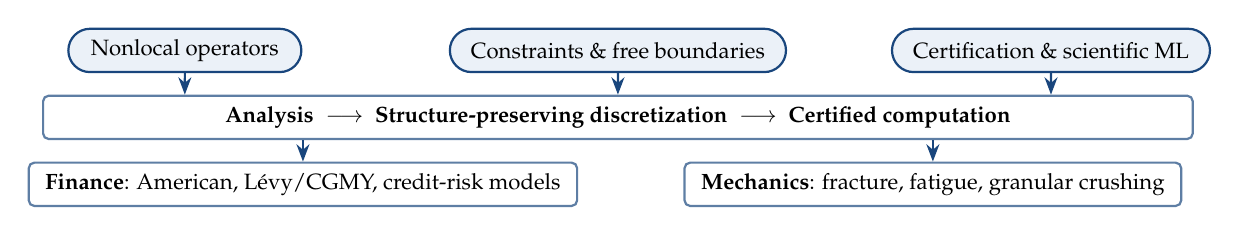
\begin{tikzpicture}[
  font=\footnotesize,
  pill/.style={rounded rectangle, draw=accent, fill=soft, thick, minimum height=5.5mm, inner xsep=7pt},
  box/.style={rectangle, rounded corners=2pt, draw=accent!70, fill=white, thick, minimum height=5.5mm, inner xsep=6pt, align=center},
  arr/.style={-{Stealth[length=2.2mm]}, accent, thick}]
  \node[pill] (nl) at (-5.5,0) {Nonlocal operators};
  \node[pill] (cs) at (0,0) {Constraints \& free boundaries};
  \node[pill] (ct) at (5.5,0) {Certification \& scientific ML};
  \node[box, minimum width=14.6cm] (lev) at (0,-0.85)
     {\textbf{Analysis} \;$\longrightarrow$\; \textbf{Structure-preserving discretization} \;$\longrightarrow$\; \textbf{Certified computation}};
  \node[box] (fin) at (-4.0,-1.7) {\textbf{Finance}: American, L\'evy/CGMY, credit-risk models};
  \node[box] (mec) at (4.0,-1.7) {\textbf{Mechanics}: fracture, fatigue, granular crushing};
  \draw[arr] (nl) -- (nl|-lev.north);
  \draw[arr] (cs) -- (lev.north);
  \draw[arr] (ct) -- (ct|-lev.north);
  \draw[arr] (lev.south -| fin) -- (fin);
  \draw[arr] (lev.south -| mec) -- (mec);
\end{tikzpicture}
\end{center}
\vspace{-10pt}

% ------------------------------------------------------------- theme 1
\section{Constrained and free-boundary evolution problems}

\paragraph{Space--time least-squares methods for parabolic obstacle problems}
With collaborators in Chile, I co-developed a space--time finite element method
for the parabolic obstacle problem
$\partial_t u+Lu\ge f,\ u\ge g,\ (\partial_t u+Lu-f)(u-g)=0$ with a general
convection--diffusion--reaction operator~$L$ \rc{J2, \emph{IMA J.\ Numer.\ Anal.}\ 2025}.
Introducing the flux $\sigma=-A\nabla u$ and the reaction force
$\lambda=\partial_t u+Lu-f$ turns the problem into a first-order system whose
variational inequality has a \emph{symmetric, bounded, coercive} bilinear form;
the discrete problem is an augmented least-squares minimization. We proved
quasi-optimality (a C\'ea--Falk lemma) for \emph{any} discrete convex set,
convergence rates on simplicial and on prismatic (Gantner--Stevenson) meshes using
positivity-preserving quasi-interpolators, and a reliable a~posteriori estimator
that drives simultaneous space--time adaptivity. For the American put, adaptivity
restores the optimal rate $O((\#\mathcal P)^{-1/2})$, compared with
$O((\#\mathcal P)^{-3/8})$ on uniform meshes.

\paragraph{Minimum-residual (DPG) methods for option pricing}
My doctoral work in computational engineering developed stable methods for
variational inequalities \rc{C1} and brought discontinuous Petrov--Galerkin
methods to option pricing, including American options solved by semismooth Newton
methods. I have since built a rigorous theory
\rc{S3,\,M2}: for the correlated $d$-asset Black--Scholes operator I proved
\emph{mesh-independent} ideal inf-sup stability for both the primal and the
ultraweak formulations---the latter without any angle or compatibility
condition, via a conforming adjoint right inverse---and constructed a
uniformly bounded one-dimensional Fortin operator, which makes the practical
method unconditionally stable and quasi-optimal. Sensitivities (Delta, Gamma,
cross-Gamma) are read directly from the first-order variables. For degenerate
and path-dependent contracts I identified the weighted space
$H^1_z=\{u: z u_z\in L^2\}$ appropriate to the interior-degenerate Asian
operator, and showed that discrete barrier monitoring is an
$L^2$-nonexpansive projection.

\paragraph{Free boundaries with solution-dependent coefficients}
In the credit-rating migration model the volatility switches across an unknown
free boundary, so the coefficients depend nonlocally on the solution itself. I
introduced a \emph{recovered-coefficient} discontinuous Galerkin method
\rc{P2} in which coefficients are evaluated on a recovered state built from
averaging, the model's own mollifier, and a computable cutoff. The recovery map
is Lipschitz into $W^{2,\infty}$ uniformly in $h$, has the exact solution as a
fixed point, and is inactive for small $h,\Delta t$. This yields an
$O(h^p+\Delta t)$ energy estimate, an estimate for the location of the
migration boundary, and a clean separation between discretization and modeling
errors.

% ------------------------------------------------------------- theme 2
\section{Structure-preserving discretization of nonlocal operators}

\paragraph{Exact Galerkin assembly for the fractional Laplacian}
Assembling the integral fractional Laplacian $(-\Delta)^s$ is the bottleneck of
nonlocal finite elements. With M.~Razzaghi and T.~N.~Vo \rc{S1, submitted to
\emph{SINUM}}, I identified \emph{why} closed-form assembly from pointwise cell
actions fails for $s\ge\tfrac12$: a discontinuous cell polynomial generates a
non-integrable endpoint singularity. Imposing the shared nodal value \emph{before}
termwise integration produces a second-order algebraic cancellation, after
which every interaction class (coincident, touching, separated) has a finite
closed form for all $0<s<1$; we proved a sharp threshold for when the raw
integrals are finite. Using a one-dimensional Faermann-type localization of the
Gagliardo seminorm, we proved optimal convergence on graded meshes for
\emph{every} $0<s<1$ under a grading condition much weaker than the one given by global interpolation, and
an $N$-independent bound on quadrature consistency. A multidimensional version
based on Lauricella-type hypergeometric functions is in progress. %CHECK authorship of 2D/3D companion

\paragraph{Tempered-stable (CGMY) dynamics}
For pricing under the CGMY L\'evy process \rc{S2} I derived exact Toeplitz
connection coefficients for exponentially conjugated tempered Riemann--Liouville
operators, applied by FFT in $O(N\log N)$. A monotonicity lemma for the Fourier
symbol gives $\operatorname{Re}\mathcal A(\xi)\ge r$, hence \emph{coercivity
whenever the interest rate is positive}; interior-supported splines make the
discrete stiffness an exact Toeplitz section, so the continuous bounds are inherited
with the same constants. I proved the fully discrete rate
$O(h^{p-Y/2}+\Delta\tau^2)$ for $Y\in(1,2)$ and validated the method on
American puts and S\&P\,500 calibrations across calm and crisis regimes.

\paragraph{Earlier foundations}
Earlier, I built spectral and meshfree tools for fractional and jump models:
wavelet collocation with exact Riemann--Liouville integrals of the basis via the
regularized beta function \rc{J1,\,J4}, de-singularized radial-basis
collocation for regime-switching tempered-stable credit-risk models \rc{J5}
and American options \rc{J7}, and adaptive shooting for stochastic boundary
value problems \rc{J6}.

% ------------------------------------------------------------- theme 3
\section{Nonlocal mechanics: fracture, fatigue, and granular crushing}

\paragraph{A well-posed field theory for quasi-brittle fracture}
With S.~Coskun and R.~Lipton \rc{J3, \emph{J.\ Mech.\ Phys.\ Solids} 2025}, we
introduced the \emph{blended} model, which couples a nonlocal (peridynamic)
constitutive law with a \emph{two-point} phase field that is an algebraic
function of the strain history, so no additional diffusion equation is needed.
The displacement--damage pair is the unique solution of a single momentum
balance (Banach fixed point in $C^2([0,T];L^\infty)$); energy balance with
nonnegative dissipation \emph{follows} from the equation of motion rather than
being imposed; and for flat cracks the failure energy factors, through
Crofton's formula, into the Griffith energy $\mathcal G_c\,\mathcal H^{d-1}$,
independently of the horizon. With only three material parameters beyond the elastic constants,
simulations reproduce cyclic load--CMOD curves of concrete beams, the
structural size effect, corner-initiated cracks, and dynamic crack branching.

\paragraph{Three-dimensional crushing and comminution}
I developed and scaled a 3D framework in which every grain of an aggregate is a
fracturing peridynamic body \rc{S5}, with nonlocal contact and friction,
self-contact between fragments of the same grain, and mesh-free wall contact
through closed-form spherical-cap volumes. Fracture and comminution then emerge
without crack tracking. The framework is verified against Hertz contact and the
Kalthoff--Winkler experiment, and it quantifies how grain shape (solid,
hollow, nonconvex) controls the strength of the aggregate; aggregates of up to
1{,}000 grains (X-ray-CT-reconstructed sand and hollow spheres) have been
simulated, with production runs on up to 1{,}600 cores. %CHECK: keep only if the CT/HPC material appears in the submitted or companion paper

\paragraph{Analysis of the computational models (ongoing)}
With Lipton's group I am closing the gap between models and codes: %CHECK role on these drafts
global $L^\infty$ well-posedness of regularized PeriDEM contact dynamics and a
unique, event-driven (Zeno-free) solution of the semi-discrete scheme with
irreversible bond breaking; a state-based blended theory with physical Poisson
ratios, separate mode-I/II damage channels, and damage--plasticity; and a
fatigue extension in which a bond-wise strain-path functional yields $S$--$N$
and Paris-type laws as consequences of the constitutive law.

% ------------------------------------------------------------- theme 4
\section{Certified computation and scientific machine learning}

\paragraph{Guaranteed bounds for neural solutions of variational inequalities}
Neural PDE solvers rarely come with error guarantees, and free-boundary
problems are where they fail most quietly. In \rc{P1} I proved and implemented
guaranteed error bounds for neural approximations of parabolic obstacle
problems. The key idea is to certify the \emph{feasible projection}
$\hat v=\max\{v,g\}$ of the network, which removes all penetration terms and all
coercivity constants of the first-order theory; the resulting majorant extends
the Apushkinskaya--Repin estimate to general coefficients and is efficient in
the natural weak norm. Every integral is evaluated with outward-rounded
Taylor-model (interval) enclosures, so the bound is mathematically guaranteed on
any partition. The constants are about $59\times$ (1D) and $237\times$ (2D) smaller
than via the estimator route, and the certificate also \emph{diagnoses} failures of penalty-based training, such as a
collapsed Lagrange multiplier near the free boundary.

\paragraph{Certifying surrogates of nonlocal pricing models}
In \rc{M1} I build query-wise accept/reject certificates for reduced-order and
neural (e.g., DeepONet) surrogates of the CGMY pricing equation. A
L\'evy--Khintchine argument gives a closed-form, parameter-explicit lower bound
on the spectrum, replacing numerical eigenvalue audits; empirical interpolation
applied to the one-variable \emph{symbol}, not to matrices, yields an
$N$-independent reduced certificate evaluated in milliseconds. In our tests the
certificate never accepted an inaccurate surrogate and detected
out-of-distribution queries far more reliably than a parameter-box rule. %CHECK final numbers

% ------------------------------------------------------------- future
\section{Research agenda for the next five years}

\paragraph{1. Certified operator learning for nonlocal and free-boundary problems}
I will combine structure-preserving discretizations (Toeplitz/FFT, closed-form assembly) with residual certificates to obtain surrogates that are
\emph{fast and verifiable} in higher dimensions: multi-asset American options,
multivariate L\'evy models, and nonlocal diffusion. Specific goals are
architectures that are feasible by construction for constrained problems,
certificates for the free boundary itself (e.g., the early-exercise boundary),
and the use of minimum-residual (DPG/least-squares) functionals as training
losses whose value \emph{is} an error bound.

\paragraph{2. Mathematical foundations of computational fracture}
Open problems from my mechanics work form a coherent analysis program:
$\Gamma$-convergence of state-based blended energies to two-channel Griffith
energies as the horizon vanishes; a continuum theory of irreversible
(hard) damage, where fixed-point methods provably fail; and convergence of the
explicit time integrators used in practice. In parallel, 3D aggregate
simulations will supply representative-volume data for multiscale constitutive
laws of crushable granular media, with uncertainty quantification.

\paragraph{3. Fast, scalable solvers for nonlocal operators}
Extending cancellation-preserving assembly to two and three dimensions calls
for compressed (hierarchical or matrix-free) treatment of far-field interactions
and Toeplitz-based preconditioners, together with adaptive space--time
least-squares and DPG methods for nonlocal variational inequalities that can be
parallelized in time.

\paragraph{Funding, students, and collaboration}
These directions fit NSF DMS (Computational and Applied Mathematics, CAREER),
DOE ASCR, and DoD (ARO, AFOSR) programs, and my MURI experience prepares me to
lead interdisciplinary proposals. Each thread has entry points for students:
undergraduates can start with Greeks, spectral methods, or particle simulations;
graduate students can pursue certification theory, nonlocal finite elements, or
fracture analysis. I release research code openly (e.g., \texttt{dpg-finance}
in C++/MFEM and \texttt{certified-neural-obstacle}), and I will continue
collaborations with LSU (Lipton), Pontificia Universidad Cat\'olica de Chile
and Universidad T\'ecnica Federico Santa Mar\'ia (F\"uhrer, Karkulik),
Mississippi State (Razzaghi), and Bath (Vo). My earlier work as a bank risk analyst
left me with a lasting interest in computations whose errors have real
consequences; it drives the emphasis on certification throughout this agenda.

% ------------------------------------------------------------- references
\vspace{-4pt}
\section*{Cited work {\normalfont\small(labels match my CV)}}
{\footnotesize
\setlength{\parskip}{0pt}
\begin{list}{}{\leftmargin=2.4em\labelwidth=2.1em\labelsep=0.3em\itemsep=0pt\parsep=0pt}
\item[\rc{J1}] D.~Damircheli, M.~Razzaghi, Time--space collocation based on fractional-order generalized Chebyshev wavelets for fractional advection problem, \emph{J.\ Comput.\ Appl.\ Math.}\ (2026) 117776.
\item[\rc{J2}] J.~J.~Carvajal, D.~Damircheli, T.~F\"uhrer, F.~Fuica, M.~Karkulik, A space--time finite element method for parabolic obstacle problems, \emph{IMA J.\ Numer.\ Anal.}\ (2025).
\item[\rc{J3}] S.~Coskun, D.~Damircheli, R.~Lipton, Quasi-brittle fracture: the blended approach, \emph{J.\ Mech.\ Phys.\ Solids} 205 (2025) 106302.
\item[\rc{J4}] D.~Damircheli, M.~Razzaghi, A wavelet collocation method for fractional Black--Scholes equations by subdiffusive model, \emph{Numer.\ Methods PDEs} 40(5) (2024) e23103.
\item[\rc{J5}] D.~Damircheli, M.~Razzaghi, S.-M.-M.~Kazemi, A.~Foroush~Bastani, A de-singularized meshfree approach to default probability estimation under a regime-switching synchronous-jump tempered stable L\'evy model, \emph{Eng.\ Anal.\ Bound.\ Elem.}\ (2023).
\item[\rc{J6}] A.~Foroush~Bastani, D.~Damircheli, An adaptive algorithm for solving stochastic multi-point boundary value problems, \emph{Numer.\ Algorithms} 74 (2017).
\item[\rc{J7}] A.~Foroush~Bastani, Z.~Ahmadi, D.~Damircheli, A radial basis collocation method for pricing American options under regime-switching jump-diffusion models, \emph{Appl.\ Numer.\ Math.}\ 65 (2013) 79--90.
\item[\rc{C1}] D.~Damircheli, M.~Bhatia, Solution approaches and sensitivity analysis of variational inequalities, \emph{AIAA SciTech} (2019).
\item[\rc{S1}] D.~Damircheli, M.~Razzaghi, T.~N.~Vo, Cancellation-preserving closed-form Galerkin assembly for the 1D integral fractional Laplacian, submitted to \emph{SIAM J.\ Numer.\ Anal.}
\item[\rc{S2}] D.~Damircheli, A B-spline Galerkin method for option pricing under the CGMY tempered stable process, submitted to \emph{SIAM J.\ Financial Math.}
\item[\rc{S3}] D.~Damircheli, DPG methods for linear Black--Scholes option pricing I: European and multi-asset extensions, submitted.
\item[\rc{S5}] D.~Bhattacharya, D.~Damircheli, R.~Lipton, Crushing, comminution and fracture: extreme particle deformation in 3D granular aggregates, submitted; arXiv:2506.05362.
\item[\rc{P1}] D.~Damircheli, Certified neural approximations for parabolic obstacle problems, preprint (2026).
\item[\rc{P2}] D.~Damircheli, Recovered-coefficient DG approximation of a credit-rating migration PDE, preprint (2026).
\item[\rc{M1}] D.~Damircheli, Residual certification of neural and reduced surrogates for CGMY pricing PIDEs, in preparation.
\item[\rc{M2}] D.~Damircheli, DPG methods for linear Black--Scholes option pricing II: Asian and barrier options, in preparation.
\end{list}
}

\end{document}
